\documentclass{beamer}

\usepackage{blindtext}
\usepackage{tcolorbox}
\usepackage{listings}
\lstset{
	frame=tb,                        % = tb to put top and bottom
	framerule=0pt,
	framextopmargin=3pt,
	framexbottommargin=3pt,
	basicstyle=\small\ttfamily,      % the size of the fonts that are used for the code
	backgroundcolor=\color{gray!10},
	numbers=none,                    % where to put the line-numbers; possible values are (none, left, right)
	stringstyle=\color{black},       % string literal style
}
\usepackage{wrapfig}
\usepackage{ragged2e}

\usetheme{Patorikku}

\title{Konobi game}
\subtitle{Software Development Method Project}
\author{Fallacara E., Indri P., Pigozzi F.}
\date{}


\begin{document}
  % Per decidere se mostrare il numero di slide oppure no.
	\setcounter{showSlideNumbers}{0}

  % Pagina di titolo.
	\frame{\titlepage}

  % Azzera il contatore dei frame e inizia a mostrarlo.
	\setcounter{framenumber}{0}
	\setcounter{showSlideNumbers}{1}

  
%\section{Introduction and rules}

  \begin{frame}{Introduction}

    \begin{tcolorbox}[colback=red!90!black!10]
      The \textbf{goal} of our project is to implement the \textbf{Konobi game} in Java, giving also the user the opportunity to choose between two interfaces: \textbf{console version} or \textbf{GUI version}
    \end{tcolorbox}

    \vspace{1em}

    \begin{block}{Tools}
      \begin{itemize}
      \item IntelliJ;
        \item OpenJDK11 and JavaFX;
        \item GitHub;
        \item Gradle: building;
        \item TravisCI: continuous integrations;
      \end{itemize}
    \end{block}

  \end{frame}


\section{Konobi Game}

  \begin{frame}{Konobi}

    Konobi is a drawless connection game for two players: \textbf{Black}
    and \textbf{White}. It's played on a square board, which is initially empty. 

    \vspace{1em}

    The top and bottom edges of the board are coloured black; the left and right edges are coloured white.

    \vspace{1em}

    \begin{centering}

      \fcolorbox{black}{yellow!70!black!40}{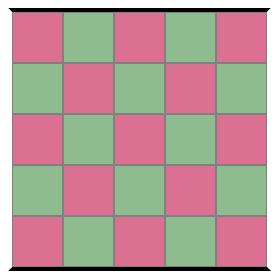
\includegraphics[width=0.35\textwidth]{img/empty.png}}

    \end{centering}

  \end{frame}



  \begin{frame}{Konobi Rules}

    \textbf{Starting with Black}, the players take turns placing stones of their own color on empty points of the board, one stone per turn.\pause

    \vspace{1em}

    Two like-coloured stones are \textbf{strongly connected} if they are orthogonally adjacent to each other, and \textbf{weakly connected} if they are diagonally adjacent to each other without sharing any strongly connected neighbour.\pause

    \vspace{1em}

    It's \textbf{illegal} to make a weak connection to a certain stone unless it's impossible to make a placement which is both strongly connected to that stone and not weakly connected to another.

  \end{frame}


  \begin{frame}{Legal and Illegal Moves}

    \begin{centering}

      Legal moves:

      \vspace{1em}

      \fcolorbox{black}{yellow!70!black!40}{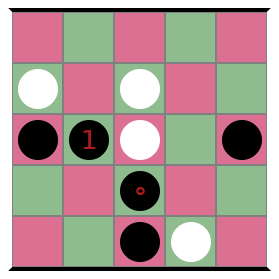
\includegraphics[width=0.25\textwidth]{img/legal1.png}}\hspace{0.1\textwidth}
      \fcolorbox{black}{yellow!70!black!40}{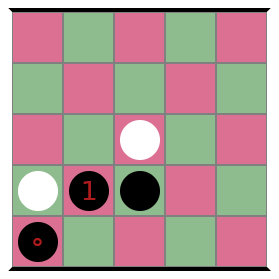
\includegraphics[width=0.25\textwidth]{img/legal2.png}}\pause

      \vspace{1em}

      Illegal moves:

      \vspace{1em}

      \fcolorbox{black}{yellow!70!black!40}{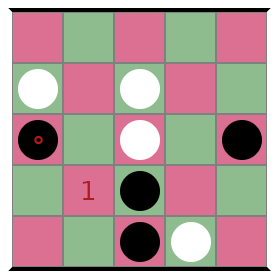
\includegraphics[width=0.25\textwidth]{img/illegal1.png}}\hspace{0.1\textwidth}%
      \fcolorbox{black}{yellow!70!black!40}{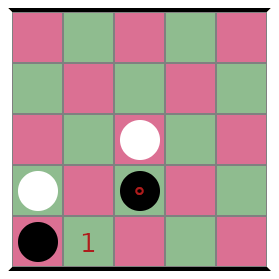
\includegraphics[width=0.25\textwidth]{img/illegal2.png}}\par

    \end{centering}


  \end{frame}



  \begin{frame}{Konobi rules Cont.}

    It's also \textbf{illegal} to form a \textbf{crosscut}, i.e., a 2x2 pattern of stones consisting of two weakly connected Black stones and two weakly connected White stones.

    \vspace{1em}

    \begin{centering}

      \fcolorbox{black}{yellow!70!black!40}{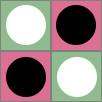
\includegraphics[width=0.25\textwidth]{img/cross.png}}

    \end{centering}\pause

    \vspace{1em}

    If a player can't make a move on his turn, he must \textbf{pass}. Passing is otherwise not allowed. There will always be a move available to at least one of the players.

  \end{frame}


  \begin{frame}{Konobi rules Cont.}

    The \textbf{pie rule} is used in order to make the game fair. This means that White will have the option, on his first turn only, to change sides instead of making a regular move.\pause

    \vspace{3em}

    The game is \textbf{won} by the player who completes a chain of his color touching the two opposite board edges of his color. \textbf{Draws are not possible}.

  \end{frame}

\section{Project Structure}

  \begin{frame}{Project Structure}

    The project is subdivided in two main packages:

    \begin{itemize}
      \item \textbf{\texttt{Core}};
      \item \textbf{\texttt{UserInterface}}.
    \end{itemize}

    \pause

    \vspace{1em}

    The \textbf{\texttt{core} package} contains all the elements concerning the functional logic of the game.

    \pause

    \vspace{1em}

    The \textbf{\texttt{UI} package}, on the other hand, contains all the elements that are used to create the two different user interfaces: \textbf{command line} and \textbf{desktop interface}.

  \end{frame}



\section{Core Package}

  \begin{frame}{Building Blocks}

    \texttt{\textbf{Cell}} class is the fundamental building block of the game engine. It is associated to a \textbf{\texttt{Colour}}, and has a \textbf{\texttt{Point}} for the coordinates.

    \vspace{1em}

    \textbf{\texttt{Board}} class is a collection of \textbf{\texttt{Cell}}s, and implements the \textbf{\texttt{Iterable}} interface. It conveys a notion of geometrical arrangement among the \textbf{\texttt{Cell}}s.

    \vspace{1em}

    \textbf{\texttt{Player}} class represents each of the two players.

  \end{frame}



  \begin{frame}{Building Blocks - TDD}

    \begin{centering}

      \fcolorbox{black}{yellow!70!black!40}{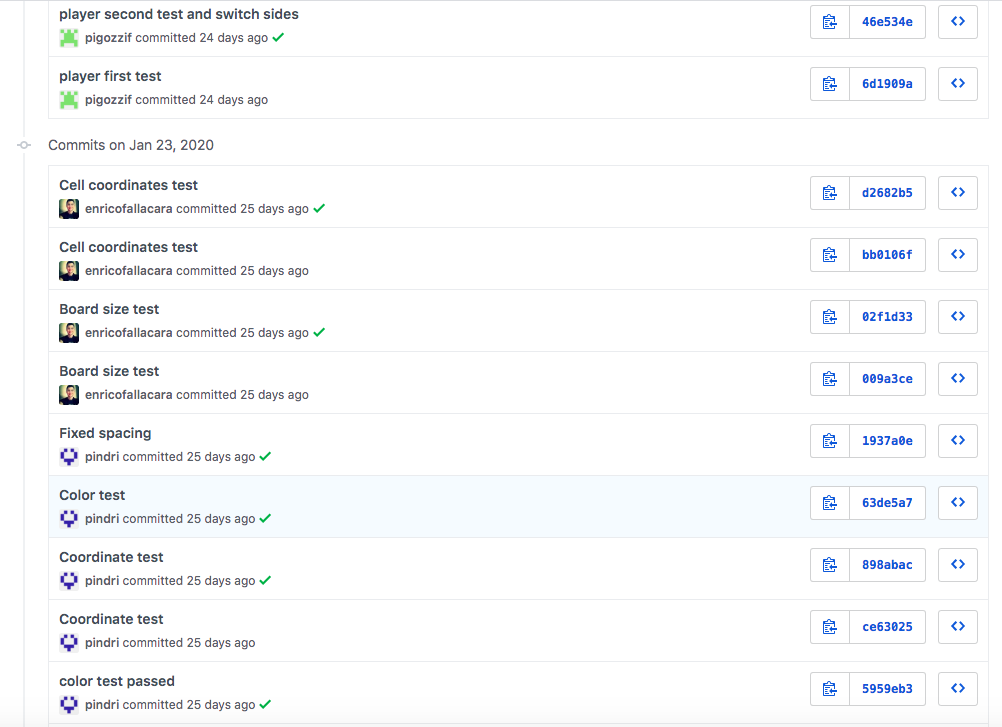
\includegraphics[width=0.75\textwidth]{img/TDD.png}}

    \end{centering}

    \vspace{1em}

    \textbf{Test Driven Development} was adopted from the very onset, committing after every red-light/green-light pattern.

  \end{frame}



  \begin{frame}{SRP and Board}

    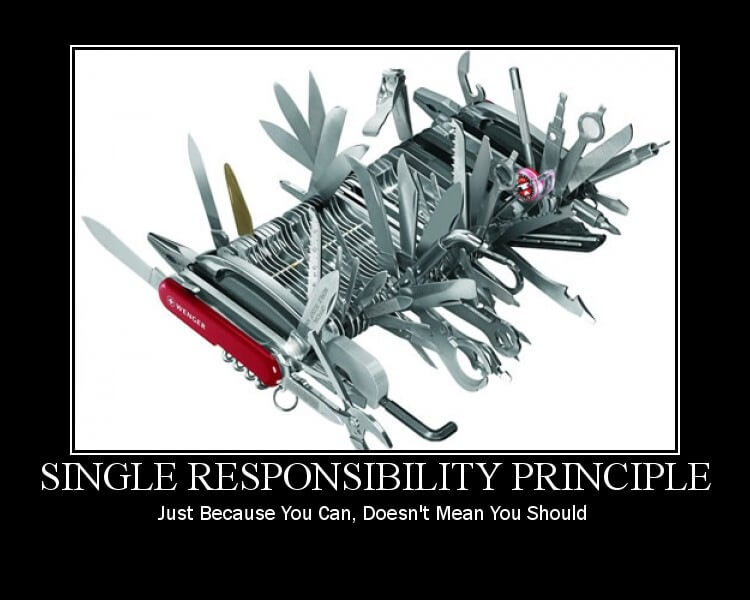
\includegraphics[height=0.35\textwidth]{img/singleresponsibilityprinciple.jpg}
    \fcolorbox{black}{yellow!70!black!40}{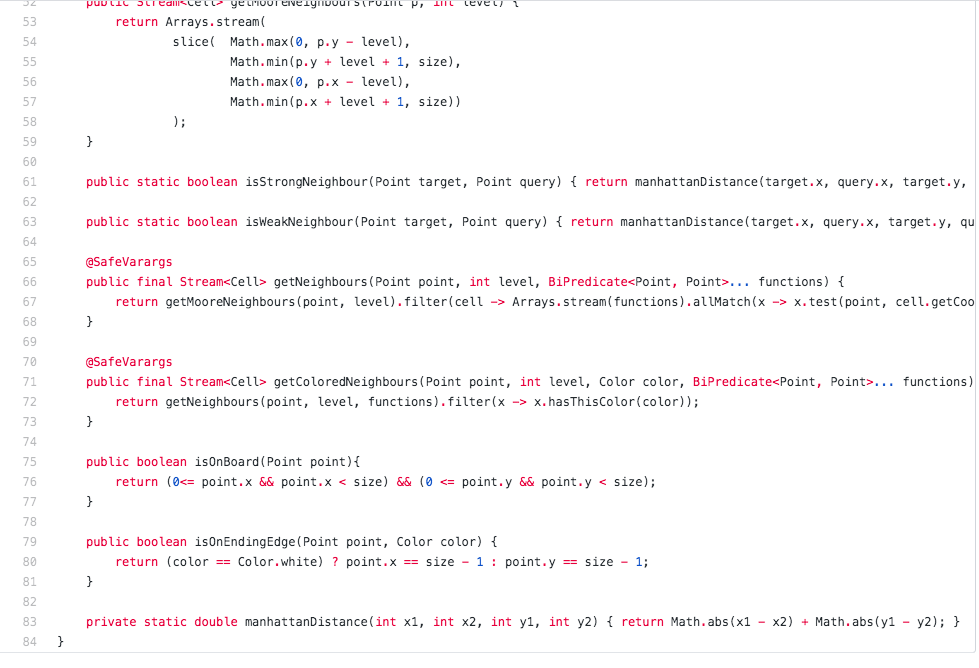
\includegraphics[height=0.35\textwidth]{img/Board.png}}

    \vspace{3em}

    \textbf{\texttt{Board}} class was doing too much, so we performed a \textbf{refactor}...

  \end{frame}



  \begin{frame} {Neighbourhood}

    ...and created the \textbf{\texttt{Neighbourhood}} class. It shows a \textbf{Monostate Pattern}, having only static methods to compute different flavours of neighbourhoods from an instance of \textbf{\texttt{Board}} and a target \textbf{\texttt{Point}}.

  \end{frame}



  \begin{frame} {Building Blocks Cont.}

    \textbf{\texttt{StatusSupervisor}} is in charge of holding the state of the game, and updating it whenever it changes (new move, pass rule, pie rule).

    \vspace{1em}

    It is employed as an interface between the \textbf{\texttt{UI}} module and the \textbf{\texttt{core}} module, allowing the two to communicate without knowing anything of each other.

  \end{frame}



  \begin{frame} {Rules}

    The package \textbf{\texttt{Rules}} contains the true logic of the game. We started off by defining a class per rule, later to realize there was room for abstraction...

    \vspace{1em}

    ...we introduced \textbf{\texttt{StatusSupervisor}} as a \textbf{Preserve Whole Object}, and allowed each of the classes to implement the \textbf{\texttt{Rule}} interface.

    \vspace{1em}

    Each \textbf{\texttt{Rule}} can be queried by passing a \textbf{\texttt{Supplier}} for it to the \textbf{\texttt{Rulebook}}.

  \end{frame}



  \begin{frame} {Rules Cont.}

    \textbf{\texttt{ValidPositionRule}} class had something wrong...

    \vspace{1em}


    \raisebox{2.5em}{\fcolorbox{black}{yellow!70!black!40}{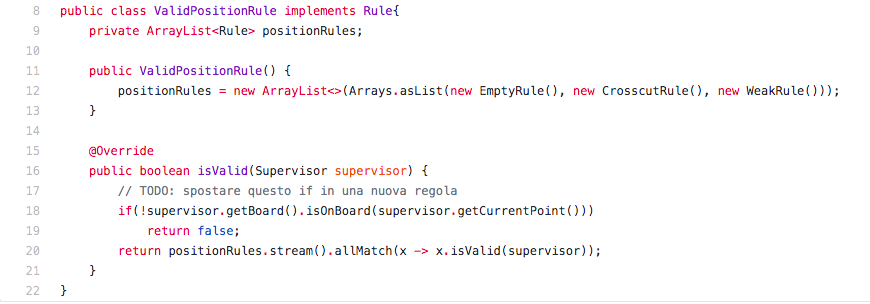
\includegraphics[width=0.5\textwidth]{img/validpositionrule.png}}}\pause
    \hfill
    
\includegraphics[width=0.45\textwidth]{img/openclosedprinciple.jpeg}

    \pause

    \vspace{1em}

    Violation was solved creating \textbf{\texttt{ValidPositionRulesFactory}} class, which follows the \textbf{Factory Pattern}.

  \end{frame}


  \begin{frame} {Konobi}

    \begin{minipage}{\textwidth}
    \begin{columns}[t]
      \begin{column}{0.40\textwidth}

        \vspace{3em}

        \justifying
        \texttt{\textbf{AbstractKonobi}} provides an abstraction for the game itself, containing functions to check and apply the various rules; it is extended by:

        \vspace{1em}

        \begin{itemize}
          \item \textbf{\texttt{KonobiConsole}};
          \item \textbf{\texttt{KonobiGUI}}.
        \end{itemize}

      \end{column}
      \begin{column}{0.50\textwidth}

        \fcolorbox{black}{yellow!70!black!40}{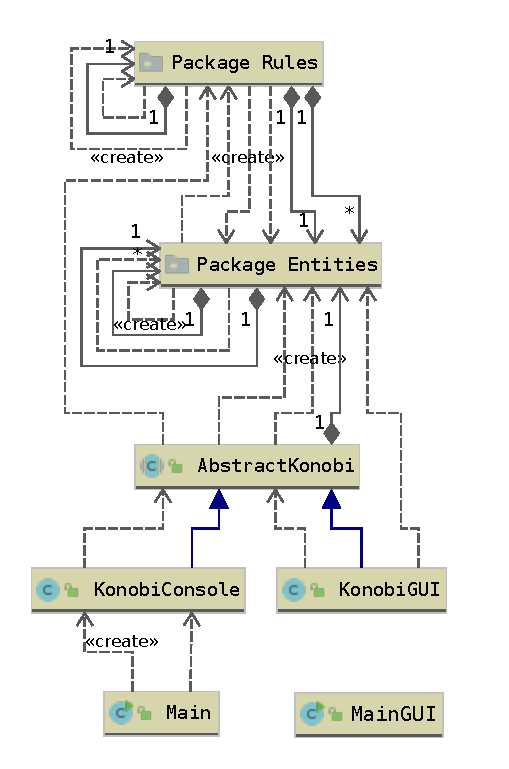
\includegraphics[width=0.9\textwidth]{uml_diagrams/core.pdf}}

      \end{column}
    \end{columns}
    \end{minipage}

  \end{frame}




\section{UI Package}


  \begin{frame}{Interacting with the game}


    \begin{minipage}{\textwidth}
    \begin{columns}[t]
      \begin{column}{0.45\textwidth}

        \justifying
        At first, we considered abstracting the console and the graphical interfaces with a common Java interface.

        \vspace{1em}
        
        We realised this was leading us to \textit{conceptualisation abuse}. 

      \end{column}
      \begin{column}{0.45\textwidth}

        \fcolorbox{black}{yellow!70!black!40}{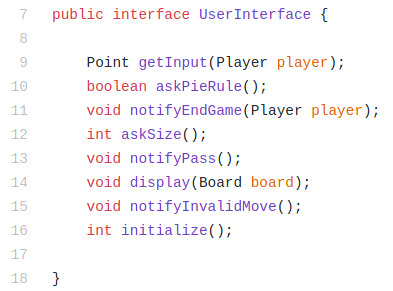
\includegraphics[width=0.9\textwidth]{img/interfaceinterface.png}}

      \end{column}
    \end{columns}
    \end{minipage}

    \vspace{2em}

    Implementation of \texttt{\textbf{UserInterface}} would have led to violations of the \textit{SRP}.

    \vspace{1em}

    The two interfaces are diverse enough, so we decided to create two distinct packages with different classes.
  \end{frame}
  


  \begin{frame} {Common elements}

    The two interfaces do have something in common. They use the same \texttt{\textbf{Messages}} and they both implement an \textbf{\texttt{InputHandler}} to ask the users for input and a \textbf{\texttt{MessageWriter}} to communicate with them.

    \vspace{1em}

    \begin{centering}

      \fcolorbox{black}{yellow!70!black!40}{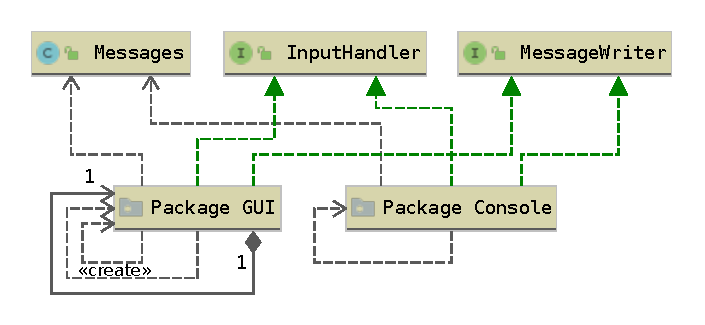
\includegraphics[width=0.75\textwidth]{uml_diagrams/UI.pdf}}

    \end{centering}

  \end{frame}




  \begin{frame}{Console User Interface}

    \textbf{\texttt{ConsoleBoardWriter}} handles the display of cells using \textbf{\texttt{ConsoleCellRepresentation}} to map the cell \textbf{\texttt{Colour}} to a symbol (convenient to avoid confusion with black/white console backgrounds).

    \vspace{1em}

    \begin{centering}

      \fcolorbox{black}{yellow!70!black!40}{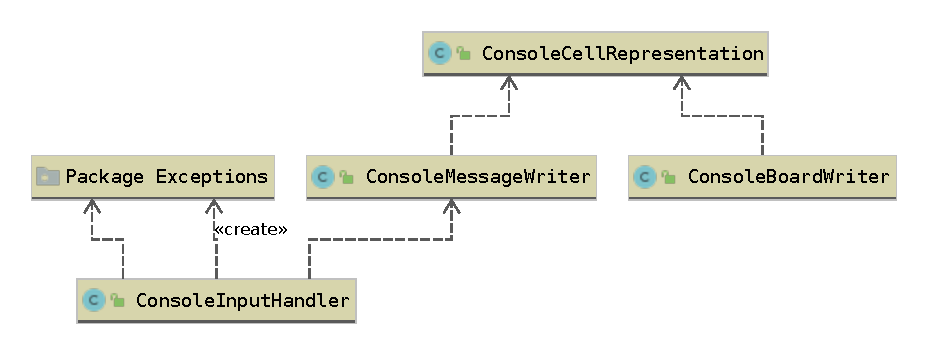
\includegraphics[width=0.75\textwidth]{uml_diagrams/Console.pdf}}

    \end{centering}

  \end{frame}



  \begin{frame}{Graphical User Interface}


    The \textbf{\texttt{GUI}} class implements the game flow in a \texttt{JavaFX} application. \textbf{\texttt{GUIBoardWriter}} deals with the creation of an empty grid and its update after each move.

    \vspace{1em}

    The \textbf{\texttt{Events}} package defines events for the rules (pie, pass and end-game rules); the events are processed by the \textbf{\texttt{Handlers}} package, which handles mouse inputs as well.

    \vspace{1em}

    At each mouse input, \textbf{\texttt{GUIMouseInputHandler}} fires the rule events using \textbf{\texttt{EventsFactory}}.

  \end{frame}



  \begin{frame}{Long method smell in GUI?}

    The \textbf{\texttt{GUI}} class is quite long: should this be regarded as a \textit{Long method smell}?

    \vspace{1em}

    \begin{centering}

      \fcolorbox{black}{yellow!70!black!40}{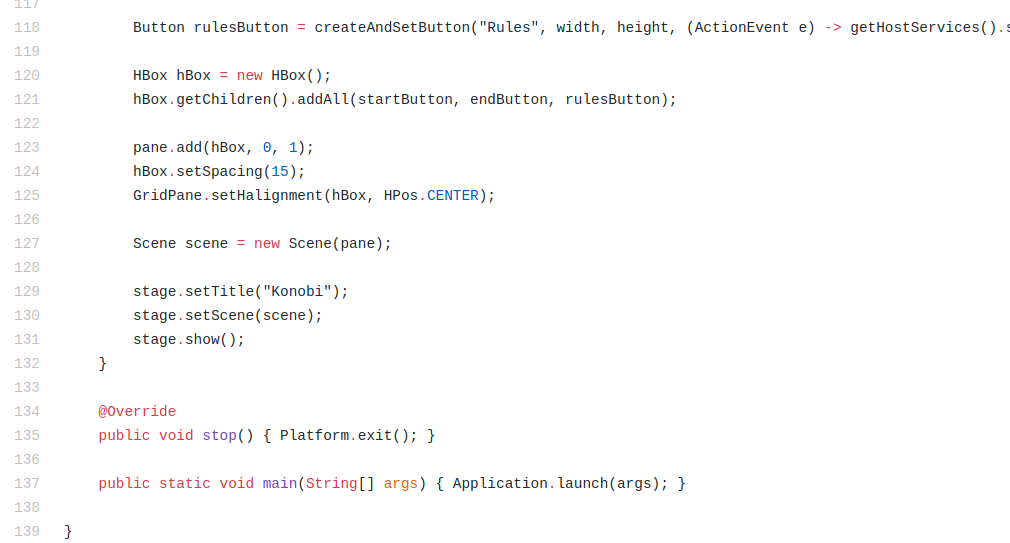
\includegraphics[width=0.75\textwidth]{img/guilongsmell.png}}

    \end{centering}

    \vspace{1em}

    \texttt{JavaFX} applications are very verbose and (moderately) long methods should not be alarming.

  \end{frame}



  \begin{frame}[fragile]{Starting game}

    For portability, the project is shipped with the \texttt{\textbf{gradlew}} (\texttt{\textbf{gradlew.bat}} for Windows) executable to run the code without manually handling dependencies.

    \vspace{2em}

    The console version of the game can be started using:

    \begin{lstlisting}
 > ./gradlew runConsole
    \end{lstlisting}

    \vspace{1em}

    \pause

    The GUI version of the game can be started using:

    \begin{lstlisting} 
 > ./gradlew runGUI
    \end{lstlisting}

  \end{frame}


  \begin{frame} {Thanks for your attention}

    Thanks for your attention!

    \vspace{2em}

    And now, let's test the project with a live demo.


  \end{frame}

\end{document}
